% \chapter{Expansion Devices}
\chapter{伸缩装置}
\label{chp:expansion-devices}
% Bridge elements are subjected to various loads, including traffic and environmental loads that result in movement of bridge elements. One of the key factors affecting the service life of bridges is how to address thermal expansion and contraction of the bridge elements. This design issue is handled in two distinct ways. One option is to provide expansion joints at designated locations within the superstructure. By doing so, the designer forces the entire thermal deformation to take place at these discrete locations. The other option is to make the superstructure and deck continuous and assume that the thermal movement will be accommodated by the flexibility of the substructure, such as with the use of integral abutments. In such cases, the joint is usually moved away from the bridge abutment and placed near the end of the approach slab.
桥梁\gls*{element}承受各种载荷,包括导致桥梁\gls*{element}移动的交通和环境载荷。 影响桥梁\gls*{servicelife}的关键因素之一是如何解决桥梁构件的热胀冷缩问题。 这个设计问题以两种不同的方式处理。 一种选择是在上部结构的指定位置提供伸缩缝。 通过这样做,设计者迫使整个温度变形发生在这些离散的位置。 另一种选择是使上部结构和桥面板连续,并使温度变形通过下部结构的柔度来调节,例如使用整体桥台。 在这种情况下,接缝通常会从桥台移开,并放置在引板板末端附近。

% This chapter provides essential information for enhancing the service life of bridge expansion joints. The process begins with developing an understanding of the types of bridge joints that may be considered for a particular project. The viable expansion joint types are further evaluated for factors that adversely affect their service life, and individual strategies are then developed to mitigate these adverse effects. The overall strategy selection is then developed, blending these individual strategies that are sometimes in conflict. The components of an overall strategy should include:
本章提供了提高桥梁伸缩缝\gls*{servicelife}的基本信息。该过程首先要了解特定项目可能考虑的桥梁接缝类型。对可行的伸缩缝类型进一步评估对其\gls*{servicelife}产生不利影响的因素,然后制定单独的策略来减轻这些不利影响。 然后制定整体战略选择,融合这些有时会发生冲突的个别战略。 总体战略的组成部分应包括:

\begin{itemize}
  % \item Identification of appropriate design methodologies,
  \item 确定适当的设计方法;
  % \item Selection of durable expansion device types considering life-cycle costs,
  \item 考虑生命周期成本选择耐用的膨胀装置类型;
  % \item Specification of best practices for construction, and
  \item 施工最佳实践的规范;
  % \item Development of an effective maintenance plan.
  \item 制定有效的维护计划。
\end{itemize}

% \cref{sec:expansion-joint-description} provides a general description of the different types of expansion devices used in practice, as well as their various advantages and disadvantages. \cref{sec:factors-joints-life} discusses reported potential factors that could affect the service life of the different expansion devices, and \cref{sec:strategy-joints-life} provides strategies for enhancing expansion device service life.

\cref{sec:expansion-joint-description} 给出了实践中使用的不同类型的伸缩装置的一般描述,以及它们的各种优缺点。\cref{sec:factors-joints-life} 讨论了已报告的可能影响不同伸缩装置\gls*{servicelife}的潜在因素,\cref{sec:strategy-joints-life} 给出了延长伸缩装置\gls*{servicelife}的策略。

\section{Description of Various Expansion Joint Devices}\label{sec:expansion-joint-description}
% There are many types of expansion joints to better meet the needs of a wide array of bridge types. However, it is important for the designing engineer to select the proper expansion joint, as this is the most crucial step in enhancing the service life of an expansion device. When selecting the proper expansion device it is important to consider the total anticipated displacements, bridge skew, and other special considerations, such as proprietary system requirements and accommodations for deicing agents, etc.
伸缩缝有多种类型,可以更好地满足各种桥梁类型的需求。然而,设计工程师选择合适的伸缩缝非常重要,因为这是提高伸缩装置\gls*{servicelife}的最关键步骤。 在选择合适的伸缩缝时,重要的是要考虑总的预期位移、桥梁斜交程度和其他特殊考虑因素,例如特有系统要求和对除冰剂的适应性等。

% Following are characteristics of an ideal expansion joint (Lee 1994):
以下是理想伸缩缝的特征 \cite{lee1994b}:
% \begin{itemize}
%   \item Accommodate thermal expansion and contraction,
%   \item Accommodate movement due to traffic-induced loads,
%   \item Provide a smooth ride,
%   \item Prevent the creation of hazards and safety issues,
%   \item Accommodate needs during snow removal,
%   \item Prevent leaking of moisture and other chemicals to elements below the superstructure,
%   \item Have a long service life,
%   \item Be maintenance-free or require minimal maintenance, and
%   \item Be cost effective.
% \end{itemize}
\begin{itemize}
  \item 适应热胀冷缩;
  \item 适应车辆荷载引起的位移;
  \item 提供顺畅的乘车体验;
  \item 防止产生危险和安全问题;
  \item 满足除雪期间的需求;
  \item 防止水分和其他化学品泄漏到上部结构下方的\gls*{element};
  \item 有较长的\gls*{servicelife};
  \item 免维护或需要最少的维护;
  \item 具有成本效益。
\end{itemize}

% There are several ways to categorize expansion joint systems. One approach is to divide the various joints based on the maximum longitudinal movements that they can accommodate. There are many different joint types and often the terminology used to describe them differs from agency to agency or manufacturer to manufacturer. Expansion joints can be classified into three categories based on the maximum longitudinal movements as follows:
有几种方法可以对伸缩缝系统进行分类。 一种方法是根据它们可以容纳的最大纵向运动来划分各种关节。 有许多不同的接头类型,用于描述它们的术语通常因机构或制造商而异。 伸缩缝根据最大纵向位移可分为以下三类:

% \begin{enumerate}
%   \item Expansion joints capable of accommodating small longitudinal movements (less than about 3 in.),
%   \item Expansion joints capable of accommodating medium longitudinal movements (between 3 and 5in.), and
%   \item Expansion joints capable of accommodating large longitudinal movements (in excess of 5 in.). 
% \end{enumerate}
\begin{enumerate}
  \item Expansion joints capable of accommodating small longitudinal movements (less than about 3 in.),
  \item Expansion joints capable of accommodating medium longitudinal movements (between 3 and 5in.), and
  \item Expansion joints capable of accommodating large longitudinal movements (in excess of 5 in.). 
\end{enumerate}

% Descriptions of the various joint types follow.
各种类型的伸缩缝描述如下:

\subsection{Expansion Joints with Small Movement Capabilities}
\subsubsection{Compression Seal}
In this type of expansion joint, the opening throughout the entire bridge deck width is filled with a neoprene
elastomeric section and forms a waterproof joint, as shown in \cref{fig:compression-seal} (Purvis 2003). The neoprene elastomeric is
installed by squeezing and inserting the seal into a preformed joint opening (Chang and Lee 2002). Steel or special
concrete materials may or may not be used to strengthen the joint face. To facilitate the movement of the joint, they
are usually made semi-hollow with internal diagonals and vertical neoprene webs (like a truss structure). However,
some types are made of closed section foam. The squeezing of the neoprene elastomeric section is meant to ensure
that it will be in compression, thereby sealing the joint. \cref{fig:compression-seal-armored} shows an armored version of a compression
seal joint. A recent trend within transportation agencies has been to eliminate the horizontal leg of the angle used and
to attach the vertical leg to the deck using shear studs. This expansion joint type allows total movement of up to 3 in.

\begin{figure}
  % \includegraphics[width=\linewidth]{graphic-file}
  \begin{minipage}{0.48\linewidth}\centering
    % \includegraphics{}
    \subcaption{plain}\label{fig:compression-seal-plain}
  \end{minipage}
  \begin{minipage}{0.48\linewidth}\centering
    % \includegraphics{}
    \subcaption{plain}\label{fig:compression-seal-armored}
  \end{minipage}
  \caption{Compression seal. (Purvis 2003)}
  \label{fig:compression-seal}
\end{figure}

\paragraph{Features}
\begin{itemize}
  \item Movement from 0.25 in. to 3.0 in. is allowed.
  \item The seal needs to be made the right size for the needed range of movement.
  \item The semi-hollow cross-section with the internal diagonal and vertical neoprene webbings forms a truss
  action, which allows the section to compress toward the sides of the joints and become watertight.
  \item Sometimes foams are used instead of semi-hollow cross-sections, which form a closed section; however, the
  movement range is the same.
  \item The compression seal fits into the sides of the joint using a lubricant material that also functions as an
  adhesive that bonds the seal to its place.
  \item Splices should be avoided in this type of seal.
\end{itemize}
\paragraph{Advantages}
\begin{itemize}
  \item Some agencies report minimal required maintenance and a good life span for these seals.
  \item This type of joint is recommended mostly for areas with moderate temperature extremes.
\end{itemize}

\paragraph{Disadvantages}
\begin{itemize}
  \item It is reported that large sustained compressive movement forces air from the seal material, which may not
  recover when the joint opening expands.
  \item Some agencies do not report good performance for this type of seal, citing damage due to debris, traffic, and
  snowplows.
  \item Leakage has also been reported shortly after installation.
  \item It has been reported to dislodge and lose compression over time.
  \item This type of joint is not recommended for extreme temperature ranges.
  \item The seal needs to be installed at relatively low temperatures or it is more difficult to install and prone to
  damage.
  \item According to some reports, the compression seal loses its capability to retain initial compression recovery
  due to loss of resilience, particularly if the movement range is large.
\end{itemize}

\subsubsection{Poured Sealants}
The poured sealant systems used today mainly consist of two parts: a polyethylene foam backer rod and a
pourable silicone sealer (Purvis 2003), as shown in \cref{fig:poured-sealant-joint-type}. The backer rod keeps the sealant from spilling
through the opening. During installation, it is very important to keep the joint edges clean so that the silicone sealant
bonds tightly. The performance of this type of joint will improve if it is poured when the ambient temperature is at
the middle of the historical range.

Traditionally, this type of joint could handle movements up to 3/16 in., but newer systems can accommodate up
to 3 in. of movement (Purvis 2003; Chang and Lee 2001).

\begin{figure}
  % \includegraphics[width=\linewidth]{graphic-file}
  \caption{Poured sealant joint type}
  \label{fig:poured-sealant-joint-type}
\end{figure}

\paragraph{Features}
\begin{itemize}
  \item Traditional systems were good for shorter spans where the movement need is 3/16 in (5 mm) or less. However, newer systems accommodate larger movements depending on the sealant material.
  \item The most common sealant used today is silicone.
\end{itemize}
\paragraph{Advantages}
\begin{itemize}
  \item This type of joint is maintaining popularity because, according to reports, newer systems are serving well if installed properly.
  \item The silicone polymer used is self-leveling and rapid-curing.
  \item The performance of this type of seal is not affected by joint walls that are not perfectly made.
  \item They are easy to repair.
  \item It is easy to remove a portion of the sealant, to clean the sides of the joint, and to refill the joint.
  \item The quick maintenance process makes traffic disruption very short.
\end{itemize}
\paragraph{Disadvantages}
\begin{itemize}
  \item The first poured seal materials were heated asphalt or coal tar products, which did not perform satisfactorily
  for many transportation agencies.
  \item Polymer materials used to have problems such as debonding, splitting, and damage from noncompressible
  debris.
  \item Earlier, damage to the deck edge also caused the joint sealant to fail.
\end{itemize}
\paragraph{Requirements}
\begin{itemize}
  \item The thickness of the silicone at the center should be no more than half the width of the joint.
  \item It is important that the bottom of the silicone does not bond to the material below.
  \item Poured sealants perform best if the seal is poured when the ambient temperature (which must be above 40oF)
  is at the middle of the historical range or the joint opening is at the midpoint.
\end{itemize}

\subsubsection{Asphaltic Plug Joint}
\cref{fig:asphaltic-plug-joint} shows a typical detail for the asphaltic plug joint. It is a simple detail that can be used with concrete deck
overlays. In this system, a center opening around the joint is prepared (about 20 in. wide and 2 in. deep), and a steel
plate is placed in the opening as shown in \cref{fig:asphaltic-plug-joint}. The asphaltic material is then placed over the steel plate to seal the
joint. The maximum movement allowed by this system is about 2 in (Pemmaraju et al. 2006; Mogawer and
Austerman 2004).

\begin{figure}
  % \includegraphics[width=\linewidth]{graphic-file}
  \begin{minipage}{\linewidth}\centering
    % \includegraphics{}
    \subcaption{Typical detail. (Mogawer and Austerman)}
  \end{minipage}
  \begin{minipage}{\linewidth}\centering
    % \includegraphics{}
    \subcaption{Commercially available details. (Courtesy D.S. Brown)}
  \end{minipage}
  \caption{Asphaltic plug joint}
  \label{fig:asphaltic-plug-joint}
\end{figure}

\paragraph{Features}
\begin{itemize}
  \item Movements less than 2 in (50 mm) are allowed.
  \item The system is suitable for concrete decks, especially when used with an overlay layer.
  \item “A popular application is on decks where a waterproof membrane, topped by bituminous (asphalt) concrete
  overlay, has been added.” (Purvis 2003)
  \item This system may work better in restricted climate conditions.
\end{itemize}
\paragraph{Advantages}
\begin{itemize}
  \item Installation and repair are easy.
  \item Installation and repair are low cost.
  \item There is a low susceptibility to snowplow damage.
  \item The system can be cold milled.
\end{itemize}
\paragraph{Disadvantages}
\begin{itemize}
  \item “This seal was developed almost exclusively for bridge deck joints without curbs, barriers, parapets, etc., and does not provide an effective method of sealing joint upturns, especially for longer decks and skewed deck
  joints where joint movement will degrade the system, resulting in early system failure.” (Purvis 2003)
  \item Some problems have also been reported, among them are softening in hot weather, debonding of the joint-pavement interface, and cracking in very cold weather.  
  \item In areas of heavy traffic volumes, this seal may rut or delaminate over time.
  \item Rapid temperature changes can damage this type of seal.
\end{itemize}

\subsubsection{Sheet Seals}
As shown in \cref{fig:sheeet-seal-eapansion-joint}, the sheet seal joint consists of a sheet of fiber-reinforced elastomeric membrane, tied to
both sides of the joints. This joint type can accommodate up to 4 in. of longitudinal movement. The kink in the
membrane allows the expansion and contraction of the joint, while keeping it watertight. This system could be used
for rehabilitation of medium-span bridges. The membrane used in this system is provided in a variety of shapes,
configurations, and sizes (Chang and Lee 2001).

\begin{figure}
  % \includegraphics[width=\linewidth]{graphic-file}
  \caption{Sheet seal expansion joint. (Yuen 2005)}
  \label{fig:sheeet-seal-eapansion-joint}
\end{figure}

\subsubsection{Sliding Plate Joint}
\cref{fig:sliding-plate-joint-system} shows a typical sliding plate joint. According to some literature (Purvis 2003), this type of joint could
also be classified as an open joint, as it does allow some level of leakage while preventing most debris from passing though the opening. This system consists of a steel plate spanning an open joint and embedded in adjoining deck
slabs. It can accommodate movements up to 3 in. Currently, these joint types can even handle larger movements,
depending on the thickness of the plate used. At present, these joint types are not used without a trough below.

\begin{figure}
  % \includegraphics[width=\linewidth]{graphic-file}
  \caption{Sliding plate joint system. (Yuen 2005)}
  \label{fig:sliding-plate-joint-system}
\end{figure}

\paragraph{Advantages}
\begin{itemize}
  \item Sliding plate joints effectively prevent debris from passing through the opening.
\end{itemize}
\paragraph{Disadvantages}
\begin{itemize}
  \item The system is noisy under traffic due to loosening over time.
  \item It is prone to safety hazards due to detaching
  \item  Anchorage problems can occur between the plate and the concrete.
  \item  Anchors can be corroded over time and are prone to fatigue damage due to traffic loads.
  \item Damage accumulated at the unsupported edge of the sliding plate causes a weak spot for traffic impact loads.
  \item  Snowplow blades can damage both the sliding plate and the anchors.
  \item The impact on the plate due to traffic loads can be increased due to deterioration of the roadway surface close
  to the joint.
  \item Sliding joints are not recommended for highways with considerable truck traffic loads.
  \item  It is not considered a watertight joint.
\end{itemize}

\subsubsection{Open Joints}
\cref{fig:open-joint-trough-armoring-angles} shows an example of an open joint with trough and armoring angles. The early versions of open joints
were constructed without trough and armoring angles; however, most departments of transportation (DOT)s are no
longer using open joints without a trough. These joint types are best suited for small movements (less than 1 in.).
Armoring provides protection against traffic impact and the trough protects bridge elements below the joints from
moisture and debris that cause deterioration.

\begin{figure}
  % \includegraphics[width=\linewidth]{graphic-file}
  \caption{An example of an open joint with trough and armoring angles.}
  \label{fig:open-joint-trough-armoring-angles}
\end{figure}

\subsection{Expansion Joints with Medium Movement Capabilities}
\subsubsection*{Strip Seals}
\cref{fig:strip-seal-expansion-joint} shows a typical configuration for a strip seal joint. The main elements are a V-shaped membrane made
using elastomeric material mechanically attached to an extruded metal piece anchored to joint edges using studs
(Purvis 2003). The maximum movement that can be accommodated by this joint system is about five in (Chang and
Lee 2002). Strip seal joints have gained popularity in recent years and most DOTs are relatively more satisfied with
strip seal joints as compared to other joint types.

\begin{figure}
  % \includegraphics[width=\linewidth]{graphic-file}
  \caption{Strip seal expansion joint.}
  \label{fig:strip-seal-expansion-joint}
\end{figure}

\paragraph*{Advantages}
\begin{itemize}
  \item  Strip seals are the most positively evaluated seals by agencies surveyed during the study done by NCHRP
  319.
  \item The seal is watertight if properly installed.
  \item Under desirable conditions, strip seals have a longer service life than any other kind of seal.
\end{itemize}

\paragraph*{Disadvantages}
\begin{itemize}
  \item Replacement is difficult.
  \item Strip seal splices should be avoided.
  \item Snowplow blades can damage the seal.
  \item Problem areas for this type of seal usually occur at locations of rapid cross section change, both in the vertical or horizontal direction of the deck, like the gutter line.
  \item During expansion, noncompressible material at tiny cracks could create membrane tears. This material can also cause ruptures, resulting in loss of water-tightness.
  \item Occasionally, the seal comes loose from the extruded metal holding piece.
\end{itemize}

\subsection{Expansion Joints with Large Movement Capabilities}
\subsubsection{Modular Expansion Joints}
Modular joints were developed to accommodate large longitudinal expansion and contraction movements by
combining multiple neoprene strip elements. Depending on the number of combined strips, modular joints can
accommodate movement from 6 to 28 in. Modular expansion joints are mainly used for bridges with more complex
movements. They consist of several metallic pieces that make them prone to fatigue. The modular expansion joint
system consists of sealer, separator beams for sealers, and support bars for separator beams. Sealers can be of strip,
compression, or sheet seal type. Separator beams are usually extruded or rolled metal shapes to join the seals in a
series. The separator beams are supported on support beams at frequent intervals (Chang and Lee 2001). \cref{fig:modular-expansion-joint}
shows a schematic of one commercially available modular joint.

\begin{figure}
  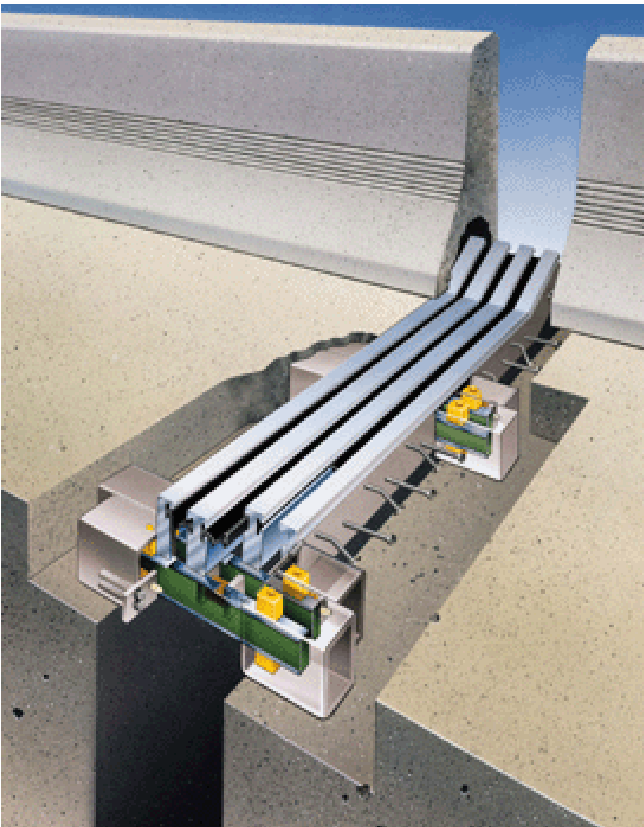
\includegraphics[width=0.5\linewidth]{modular-expansion-joint.png}
  \caption{Modular expansion joint system}
  \label{fig:modular-expansion-joint}
\end{figure}

\paragraph{Features}
\begin{itemize}
  \item The system consists of three elements: sealers, separator beams, and support bars.
  \item Modular joints are considered a closed joint system, so they protect the components below from damage due
  to water, salt, and other problems associated with deck runoff.
  \item  They are used for all types of long spans. It is the best alternative for large movements.
\end{itemize}
\paragraph{Advantages}
\begin{itemize}
  \item They can accommodate large movements over 4 in (100 mm), but the typical movement is between 6 and 24 in.
  \item They can be sized according to the magnitude of movement and have been designed to accommodate movements of more than 7 ft (very long span).
  \item Joint seals have been continuously improved.
  \item The system is improving with experience and research. New design provisions in the AASHTO LRFD Design Specifications incorporate recent fatigue related research.
\end{itemize}

\paragraph{Disadvantages}
\begin{itemize}
  \item Problems have included fatigue cracking of welds (older designs); damage to the equalizing spring, the neoprene sealer material and the support; and damage from snowplows.
  \item The system is complex and must be capable of expanding and contracting to accommodate very large movements and must remain watertight while be supported by a movable framing system.
  \item  The high initial and maintenance cost. Many DOTs have returned to using finger joints for large movements and placed additional emphasis on proper drainage.
  \item There are only two primary suppliers, which limits competition.
  \item Mixed performance results have been reported.
\end{itemize}

\paragraph{Performance Requirements for Modular Expansion Joints}
Modular expansion joints, by some agencies, are exclusively used to accommodate large movements. Water tightness and fatigue resistance are important considerations and some states have or are developing specifications to ensure these considerations.

\subsubsection{Finger Plate Joints}
\cref{fig:finger-plate-joint-system} shows a typical finger plate joint system. Two pieces of steel are anchored either to the deck or the
steel superstructure and cover the joint opening. Grooves in each of the plates fit loosely together like fingers. The
majority of the finger plate joint systems in use have a trough as shown in \cref{fig:finger-plate-joint-system} to catch water and debris and
carry it away from the superstructure to prevent deterioration (Purvis 2003; Chang and Lee 2001). A variation of this
concept is to offset the location of the finger assembly to one side of the deck opening, whereby the fingers from one
side slide over an embedded plate in the deck on the other side. The advantage of this design is that the deck opening
is covered and limits the amount of debris that can fall through.

\begin{figure}
  % \includegraphics[width=\linewidth]{graphic-file}
  \caption{Examples of a finger plate joint system.}
  \label{fig:finger-plate-joint-system}
\end{figure}

\paragraph{Features}
\begin{itemize}
  \item The system consists of finger like plates attached to both sides of the superstructure and usually includes a
  drainage trough.
  \item  It is considered an open joint system.
\end{itemize}
\paragraph{Advantages}
\begin{itemize}
  \item These joints can accommodate large movements over three in.
  \item The system experiences fewer durability problems in comparison with modular joints, and tends to have
  fewer problems than many other joints.
  \item DOTs have opted to use finger joints on longer spans.
\end{itemize}
\paragraph{Disadvantages}
\begin{itemize}
  \item The upward bending of the ends of the fingers results in increased noise, a rough riding surface, and
  occasionally broken fingers.
  \item  The most common problem is concrete deterioration around the joint.
  \item The only corrosion protection for the components below is the drainage trough.
  \item  Problems are usually caused by poor drainage trough design.
  \item Cleaning and flushing are often difficult and are rarely performed.
\end{itemize}

\paragraph{Performance Requirement s for Finger Plate Expansion Joint}

Water tightness and good drainage is an important consideration for finger plate expansion joints. Use of
appropriate slope (min 1\%) can easily address this requirement. When using finger plate expansion joints, following
the installation requirement specified by manufacture is important. Maintenance of the trough and routinely cleaning
the debris is essential when using finger plate expansion joint.


% \section{Factors and Considerations Influencing Expansion Joint Service Life}\label{sec:factors-joints-life}
\section{影响伸缩缝\glsentrytext{servicelife}的因素和注意事项}
\label{sec:factors-joints-life}
Joint performance is perhaps the most important factor affecting the deterioration of bridge elements. A leaky
joint allows salt and other chemicals to penetrate below the deck and causes many maintenance and deterioration
problems. A study conducted by the FHWA (Fincher 1983) reports that over a five-year period, more than 60\% of
joints evaluated were leaking water, and the other 40\% had problems that were actually decreasing their service lives.
Another study conducted by Wallbank in 1989 evaluated 200 concrete bridges and found leaking expansion joints to
be the major cause of bridge element deterioration.

The reduced service life of bridge expansion devices is primarily related to deficiencies, which may be load-
induced, caused by man-made or natural hazards, or result from production defects in construction processes and/or
design details, or operational procedures. These deficiencies are illustrated in the fault tree shown in \cref{fig:faulttree-expansion-joint}.

\begin{figure}
  % \includegraphics[width=\linewidth]{graphic-file}
  \caption{Expansion joint reduced service life fault tree}
  \label{fig:faulttree-expansion-joint}
\end{figure}

\subsection{Load-Induced Expansion Joint Considerations}
Load-induced bridge deck deterioration can be attributed to either loads induced by the traffic that the bridge
deck expansion device carries, or by characteristics dependent on the overall bridge system. These load-induced
factors are introduced in the fault tree provided in \cref{fig:faulttree-expansion-joint-load-induced}.

\begin{figure}
  % \includegraphics[width=\linewidth]{graphic-file}
  \caption{Load-induced deficiency fault tree.}
  \label{fig:faulttree-expansion-joint-load-induced}
\end{figure}

\subsubsection{Traffic-Induced Load Considerations}
Traffic-induced loads include the effects of truck and other vehicle traffic on the riding surface of the bridge.
Bridge deck loading, and thus the loading on the expansion devices, has a degree of uncertainty that must be
addressed during design of the bridge including vehicle weights and frequency of application, vehicle axle and tire
spacing, vehicle location on the deck, and variability in vehicle suspension systems that can affect impact
assumptions. The assumptions in loading must be carefully reviewed when establishing the criteria to be used, and checked for bridge expansion device design. Typically the service life of bridge deck expansion devices will be
affected by fatigue response to repetitive loading, overload, and wear and abrasion.

\paragraph{Fatigue}
Fatigue is caused by the repetition of applied loads that result in a degradation of the strength resistance of the
components used to resist tensile stresses that occur in expansion devices (especially in modular expansion joints and
other large movement joints).

\paragraph{Overload}
Despite weight limit regulations in most states that define load limits for permit and legal truck configurations,
overloads exceeding these limits are not specifically controlled. There are few weigh stations for checking these
loads and they are usually only found on major roadway facilities, such as Interstate highways. Enforcement of the
laws against these overloads on other facilities is limited to spot checks by code enforcement officials.

Overloads result in additional flexural stresses in bridge decks and expansion devices that can cause excessive
cracking and movements not accommodated by the original design. Heavier tire loads may also affect the wear and abrasion on the structure. Multiple applications of these loads can also affect the fatigue behavior of the deck
expansion devices.

\paragraph{Wear and Abrasion}
Wear and abrasion is typically affected by high traffic volumes, high tire loads, and the types of tires used by the
vehicles. In cold climates, tires may have enhanced features to aid in traction, such as deep grooves, studs, and
chains. These added tire features, while aiding traction, can abrade the surface of the bridge expansion joints.

\paragraph{Snow Plow}
Impacts from snow plows are special considerations that need to be addressed in the selection of expansion joints. Repeated impacts from snow plows can cause expansion devices to function incorrectly and even make driving over them unsafe.

\subsubsection{System-Dependent Loads}
System-induced loads include the effects of the bridge system configuration on the behavior of the bridge deck
expansion devices. These effects are accentuated by restraints provided through the bridge system and bridge deck
boundary conditions, and can result in significant locked-in stresses.

\paragraph{System Framing Restraint}
Boundary conditions for the longitudinal and transverse restraint of bridges can result in tension that may lead to
cracking in bridge decks under cold weather conditions. These boundary condition restraints are introduced through
design by the choices made relating to bearing types and their fixity and sliding assumptions. Fixed bearings provide
an anchor that is intended to restrict “walking” of the superstructure resulting from shrinkage and cycling of
expansion and contraction, and are usually located longitudinally near the point of zero movement of a supported
multi-span superstructure unit. These fixed bearings, used in combination with bearings designed to allow the
superstructure to either move or slide over the top of the substructure, reduce restraining forces that would otherwise
be required to resist the movement.
\paragraph{Thermal}
Temperature changes can result in changes in bridge movement, which can affect the service life of expansion
joints.

\subsection{Natural or Man-Made Hazard Considerations}
The environment to which the bridge deck is subjected can have a significant influence on the service life of
bridge decks and consequently the expansion devices.

These environmental influences include hazards from both natural and manmade sources and include effects
from areas with adverse thermal climate, coastal climates, and chemical climates, as well as from chemical properties
of the materials and outside agents, such as fire. These natural and manmade hazards are introduced in the fault tree
provided in \cref{fig:faultree-expansion-joint-hazard}.

\begin{figure}
  % \includegraphics[width=\linewidth]{graphic-file}
  \caption{Natural or man-made hazard fault tree}
  \label{fig:faultree-expansion-joint-hazard}
\end{figure}
\subsubsection{Thermal Climate}
Thermal climate influences on bridge deck expansion device service life performance are primarily due to cold
weather climates. These influences are both man-made from the application of deicing salts, and natural, in the case
of freeze/thaw.

\paragraph{Application of Deicing Salts}
Agencies in cold weather climates dealing with ice and snow on roadways and bridges have traditionally applied
deicing salts to melt the ice and snow to facilitate tire traction on their facilities. These chloride-laden compounds can
cause corrosion of expansion joint steel components.

The cross slope built into bridge decks for drainage purposes causes salt to wash down towards the bridge gutter
adjacent to the traffic railing barriers bounding the bridge. Removal equipment that scrapes snow from the bridge
deck will also deposit residual snow laden with deicing salts at this location, resulting in a very high concentration of
chlorides.

\paragraph{Freeze/Thaw}
Spalling and cracking of the concrete deck due to freeze/thaw at the sites of expansion joints could have adverse
effects on the joint-to-deck connections and possibly on the performance of the device as well.

\subsubsection{Coastal Climate}
Coastal climate influences on bridge expansion joint service life performance are primarily due to chlorides
introduced through salt spray and effects from high humidity. These influences both occur naturally.

\paragraph*{Salt Spray}
Coastal regions are subjected to a chloride-laden saltwater environment and a combination of wind and wave action that causes these chlorides to become airborne as salt spray. The susceptibility of the bridge expansion joints to these environmental influences depends on the height of the bridge deck above the water elevation. The salt spray wets the surfaces leaving a chloride residual that can cause steel components of expansion devices to corrode.

\subsubsection{Chemical Climate}
Chemical climate influences on service life performance can be attributed to corrosion-inducing chemicals or other chemicals that can have detrimental effects on exposed neoprene elements. These influences can occur naturally or can be manmade.

\paragraph*{Corrosion-Inducing Chemicals}
Corrosion-inducing chemicals can be introduced to the bridge deck and joints from adjacent industries in which residuals from pollution can attribute to reduction in bridge expansion joint service life. As an example, oil and coal burning facilities release sulfur dioxide and nitrogen oxide into the air, which causes acid rain consisting of sulfuric and nitric acids. These acids can dissolve cement compounds in the cement paste and calcareous aggregates, and leave crystallized salts on concrete surfaces that can lead to spalling and the corrosion of reinforcing bars at the site of expansion devices, as well as components of the joints themselves.

\subsection{Production and Operation Bridge Deck Considerations}
Decisions made for the production of bridge expansion devices and activities during its operation can have a significant influence on the service life of bridge expansion joints. These production and operation influences are introduced in the fault tree provided in \cref{fig:faulttree-expansion-joint-operation}, and include decisions made during the design and detailing of the bridge expansion joints, and decisions regarding the quality of construction, the level of inspection and testing performed during operations, and maintenance implementation.

\begin{figure}
  % \includegraphics[width=\linewidth]{graphic-file}
  \caption{Production/operation and design/detailing defects fault tree}
  \label{fig:faulttree-expansion-joint-operation}
\end{figure}

\subsubsection{Design and Detailing Bridge Deck Considerations}
Decisions made during the design and detailing phase of a bridge project can significantly impact the service life of the bridge. It is incumbent upon designers to understand the implications of these decisions in order to make rational choices that will improve the service life of bridge expansion devices.

\subsubsection{Construction}
Attention to good practices during construction and installation is crucial to the long-term durability of expansion devices. Well-qualified, trained and executed workmanship increases productivity, reduces material waste, and provides expected service life. Proper use of test methods is needed to ensure that quality expansion joints are achieved.

\subsubsection{Maintenance Plan—Monitoring of Condition}
An effective maintenance plan must include provisions to adequately monitor the structure in order to identify deficiencies at an early age so that appropriate repairs can be performed before the deficiency propagates into an irreparable condition. The plan should address proper inspection, collection of data, and prompt action upon reported deficiencies.

\subsubsection{Inspection Requirements and Intervals}
Inspection is a valuable tool for increasing the service life of bridges. Identification of deterioration at an early stage is essential to providing corrective actions in a timely manner in order to maximize the owner’s investment in the structure. The scope and interval of these inspections should be calibrated based on bridge expansion device performance history for the applicable deck hazard exposures. Inspection personnel should be properly trained to identify this deterioration.

\section{Overall Strategies for Enhanced Bridge Expansion Joints Service Life}\label{sec:strategy-joints-life}
Providing bridge expansion joints with enhanced service life requires a full understanding of the potential deterioration mechanisms. These mechanisms are associated with load-induced conditions, local environmental hazards, production-created deficiencies, and lack of effective operational procedures. This process is presented in this section.

The intention of this section is to provide guidelines for selecting the most appropriate individual strategy to achieve the desired service life.

\subsection{Design Methodology}
With limited funds available for bridge construction, first-cost economy is often an overriding factor in critical bridge joint selection decisions. However, to take advantage of the long-term advantages of durable expansion joints, service life enhancement strategies must apply a cascading series of economy, design, construction, and maintenance measures. The success of the strategy selection process is dependent on the ability to predict service life and the incorporation of best practices to enhance service life.

\subsection{Expansion Joint System Selection}
In general, selection of bridge expansion joints is historically based on locally accepted construction practices and procedures, which result in an economical deployment. Proposed enhancements to these systems would need to be assessed on the specific long-term performance of these systems. As noted in \cref{sec:factors-joints-life}, there are numerous deficiencies that result in a reduction of service life, and these conditions may not necessarily occur at the specific project site under consideration. It is the design engineer’s responsibility to understand local practice and its performance history, and to perform sufficient investigation of the project site, its environment, and other design conditions prior to selecting an expansion joint and its potential enhancements.


% \subsection{Life-Cycle Cost Analysis (LCCA)}
\subsection{\texorpdfstring{\acrfull*{lcca}}{全生命周期成本分析}}
Once a series of strategies has been developed, the evaluation of these strategies is performed through a life-cycle cost analysis. \acrlong*{lcca} provides an assessment of the overall long-term cost of a strategy throughout the target service life of the structure. \acrlong*{lcca} is discussed in detail in \cref{chp:lcca} of this guide.

The analysis should consider all costs associated with the construction required, implementation trials and testing, and all future maintenance actions required through the life of the structure.

\subsection{Construction Practice Specifications}
Once the bridge expansion joint system is selected, a proper set of specifications must be developed to ensure the appropriate standard of care is used during construction. It should be noted that many agencies and manufacturers have specific requirements for temperature setting for expansion joints to allow maximum range of movements, which need to be considered during design and construction.


\subsection{Maintenance Plan}
An effective maintenance plan must be developed to ensure the assumptions regarding maintenance upkeep made in the bridge expansion joint selection process are properly identified for staff and budget requirements. If the bridge owner cannot commit to such a program, then strategies for low maintenance life-cycle costs should be recommended.

\subsection{Retrofit Practices for Expansion Devices}
Expansion joints in bridges are not typically retrofitted as it is common practice to replace the joints when they reach the end of their service life. Due to the perishable nature of these expansion joints, it is important that they beproperly maintained in order to maximize the life of such devices.

\subsection{Technology Tables}
The following technology table is provided to summarize service life and durability issues related to expansion joints, and to aid the designing engineer in selecting the proper expansion device. \cref{tab:bridge-joints-technology} provides service life issues related to most expansion joints used in practice. The information could be used in several different ways at the design or maintenance level. The purpose of the technology table is to identify the most common types of service life problems encountered in commonly used expansion joints, and this information can subsequently be utilized to provide possible solutions to service life problems encountered with expansion joints.

\begin{table}
  % \caption{Bridge Joints Technology Table}
  \caption{Bridge Joints Technology Table}
  \label{tab:bridge-joints-technology}
  % \input{tables/bridge-joints-technology}
\end{table}

Review of the technology tables indicates that the following modes of failure are observed when various expansion joints are used:
\begin{itemize}
  \item Damage to various expansion joint components, such as steel armors, due to snowplow usage;
  \item Inadequate design, installation, and maintenance;
  \item Accumulation of debris, leading to limited movement;
  \item Lack of timely maintenance;
  \item Limited service life; and
  \item Leakage.
\end{itemize}

The ultimate consequence of these service life problems is that joints start leaking and causing damage to bridge elements below the deck.

% \subsection{Strategy Table for Expansion Joints}
\subsection{伸缩缝策略表}
% Selecting the appropriate expansion device for the required movement range is the most critical step in enhancing the service the life of these joints. \cref{tab:strategy-table-expansion-joints} summarizes the information presented in this chapter and proposes recommended strategies when expansion devices are to be used. The table is intended to serve as a guide to the designer in selecting bridge expansion devices.
为适应桥梁的运动与变形选择合适的伸缩装置是提高这些接缝使用寿命的最关键步骤。\cref{tab:strategy-table-expansion-joints}总结了本章中提供的信息,并提出了使用伸缩装置时的建议策略。该表旨在作为设计人员选择桥梁伸缩装置的指南。

\begin{table}
  % \caption{Strategy Table for Expansion Joints}
  \caption{伸缩缝策略表}
  \label{tab:strategy-table-expansion-joints}
  % \begin{tblr}{
  colspec={X[l] X[l] X[l]},
  row{1,2}={m,c,bg=genfg,fg=white,font=\bfseries,guard}
}
最大伸缩量(\unit{mm})& 策略 & 潜在\glsentrytext{deterioration}模式 & 提高\glseentrytext{servicelife}的选项 & \Se\\
\end{tblr}

\end{table}
